\customlink{The_geomagnetic_field}
\chapter{The geomagnetic field}
\index{geomagnetic!field}
\index{magnetic!field!Earth's}



One of the major efforts in paleomagnetism has been to study
ancient geomagnetic fields. Because human measurements extend back about a millenium, measurement of ``accidental'' records provided by  archaeological or geological materials remains the only way to investigate ancient field behavior.  Therefore it is useful for students of paleomagnetism to understand something about the present geomagnetic field.  In this chapter we review the
general properties of the Earth's magnetic field.  

The part of the geomagnetic 
field of interest to paleomagnetists is generated by convection currents in the liquid outer core
of the Earth which is composed of iron, nickel and some unknown lighter
component(s). The source of energy for this convection is not known for certain, but is thought to be partly from cooling of the core and partly from the bouyancy of the iron/nickel liquid outer core caused by freezing out of the pure iron inner core.    Motions of this conducting fluid  are 
controlled by the bouyancy of the liquid, the 
spin of the Earth about its axis and by the interaction of the conducting fluid with the magnetic field (in a horribly non-linear fashion).  Solving the equations for the  fluid motions and resulting magnetic fields is a challenging computational task.   Recent numerical models, however, show that  such magnetohydrodynamical systems can   produce self-sustaining dynamos which  create
enormous external magnetic fields.  



\section {Components of magnetic vectors}
\label{sect:comp}

The magnetic field of a dipole aligned along the spin axis and centered in the Earth (a so-called 
\index{geocentric axial dipole}%
{\it geocentric axial dipole}, or GAD) is shown in Figure~\ref{fig:coord}a. [See Chapter 1  for a derivation of  how to find the radial and tangential components of such a field.]   By convention, the sign of the Earth's dipole is negative, pointing toward the south pole as shown in Figure~\ref{fig:coord}a and magnetic field lines point toward the north pole.  They point  downward in the northern hemisphere and upward in the southern hemisphere.  
\begin{figure}[htb]
%\epsfxsize 14.5cm
  %\centering \epsffile{EPSfiles/components.eps }
\centering  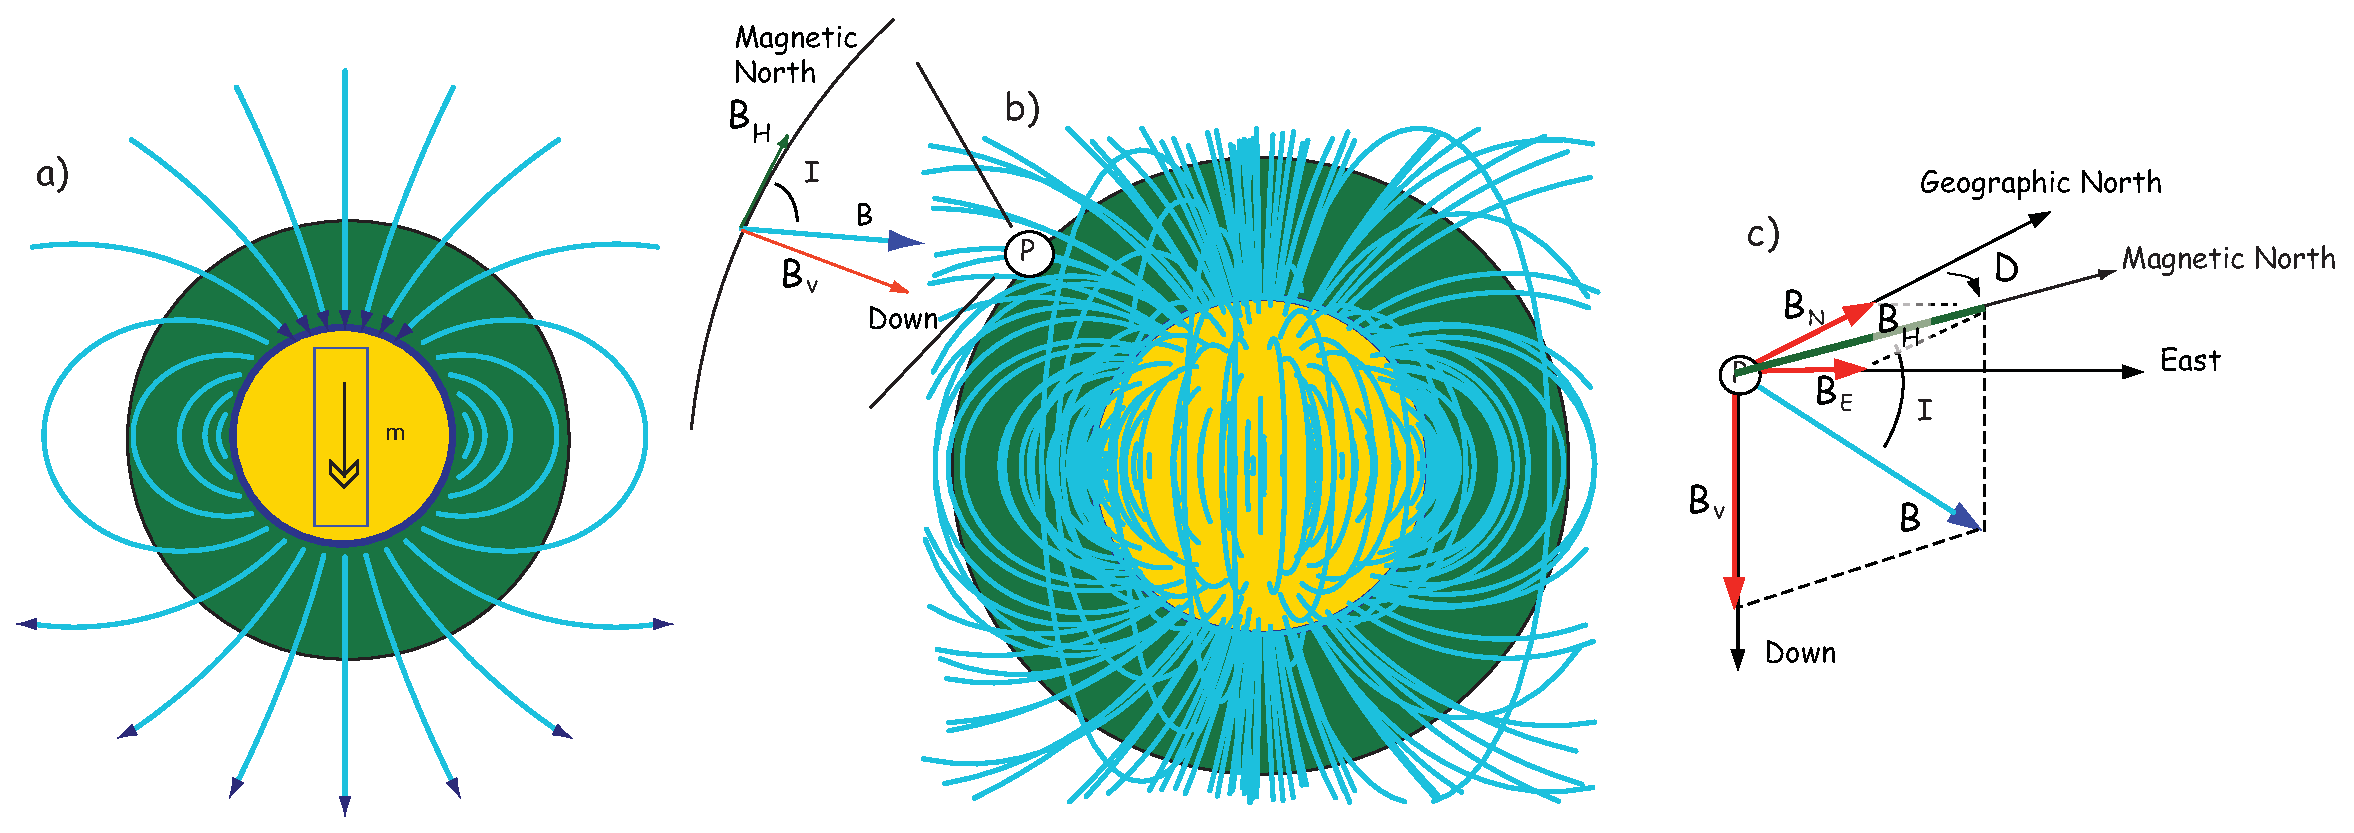
\includegraphics[width=14.5 cm]{EPSfiles/components.eps}
\caption{a) Lines of flux produced by  a geocentric axial dipole.  b) Lines of flux  of the geomagnetic field of 2005.   At point P the horizontal component of the  field $B_H$, is directed toward the magnetic north.  The vertical component $B_V$ is directed down and the field makes an angle $I$ with the horizontal, known as the
%\index{inclination}%
inclination.  c) Components of the geomagnetic field vector $\B$.  The angle between the horizontal component (directed toward magnetic north and geographic north is the 
declination $D$.) [Modified from Ben-Yosef et al., 2008b.] 
}
\label{fig:coord}
\end{figure}
\nocite{benyosef08b}

\index{magnetic!field!components}
Although dominantly dipolar, the  geomagnetic field is not perfectly modeled by a geocentric axial dipole, but is somewhat more complicated (see Figure~\ref{fig:coord}b).  At the point on the surface labeled `P', the geomagnetic field points nearly north and down at an angle of approximately 60$^{\circ}$.   
Vectors in three dimensions are described by three numbers and in many paleomagnetic applications, these are two angles ($D$ and $I$) and the  strength ($B$)  as shown in  Figure~\ref{fig:coord}b and c.  The angle from the horizontal plane  is  the
\index{inclination}%
 {\it inclination} $I$; it  is positive downward and ranges from +90$^{\circ}$ for straight down to -90$^{\circ}$ for straight up.   If the geomagnetic field were that of a perfect GAD field, the horizontal component of the magnetic field ($B_H$ in Figure~\ref{fig:coord}b)  would point directly toward geographic  north.  In most places on the Earth there is a deflection away from geographic north and  the angle between geographic and magnetic north is the
\index{magnetic!declination}%
 {\it declination}, $D$ (see Figure~\ref{fig:coord}c).  $D$ is measured positive clockwise from  North  and  ranges from $0 \rightarrow 360^\circ$.   [Westward declinations can also be expressed as negative numbers, i.e., 350$^{\circ}$ = -10$^{\circ}$.]   The vertical component ($B_V$  in Figure~\ref{fig:coord}b,c) of the geomagnetic field at P, is given by 

\begin{equation}
B_V = B \sin I,
\label{eq:Bv}
\end{equation}   
\noindent and the horizontal component $B_H$  (Figure~\ref{fig:coord}c) by
\begin{equation}
B_H = B \cos I.
\label{eq:Bh}
\end{equation}  

\noindent    $B_H$
can  be  further resolved into north and east components ($B_N$ and $B_E$ in Figure~\ref{fig:coord}c) by


\begin{equation}
 B_N=B \cos I \cos D \hskip 1em \hbox{ and } \hskip 1em B_E=B \cos I \sin D .
\label{eq:BnBe}
\end{equation}





Depending on
the particular problem, some 
\index{coordinate systems}%
coordinate systems are more suitable to
use because they have the symmetry of the problem built into them.    We have just defined a coordinate system using two angles and a length ($B,D,I$) and the equivalent 
\index{coordinate systems! Cartesian}%
Cartesian coordinates of  ($B_N, B_E, B_V$). We
will need to convert among them at will.  There are many names for the Cartesian coordinates. In addition to north, east and down, they  could also be $x,y,z$ or even
 $x_1, x_2$ and $x_3$. 
The convention used in
this book is that axes are denoted $\X_1, \X_2, \X_3$, while the components
along the axes are frequently designated $x_1, x_2, x_3$.  In the geographic frame of reference,
positive $\X_1$ is to the north, $\X_2$ is east and $\X_3$ is vertically 
down in keeping with the right-hand rule.    To convert from  Cartesian coordinates to angular coordinates ($B,D,I$):

\beq
B = \sqrt{x_1^2 +x_2^2 + x_3^2}, \hskip 1em
D=\tan^{-1} {x_2\over{x_1}}, \hbox{ and }
I=\sin^{-1} {x_3\over B}.
\label{eq:DI}
\eeq

\noindent Be careful of the sign ambiguity of the tangent function. You may well end up
in the wrong quadrant and have to add 180$^{\circ}$; this will happen if both $x_1$ and $x_2$ are negative.  In most computer languages, there is a function {\bf atan2} which takes care of this, but most hand calculators will not.     Remember that most computer languages expect angles to be given in radians, not degrees, so multiply degrees by $\pi/180$ to convert to radians.  Note also that in place of $\B$ for magnetic induction with units of tesla as  a measure of vector length, (see Chapter 1), we could also use $\H$,  $\M$ ( both Am$^{-1}$) or $\m$ (Am$^2)$ for magnetic  field, magnetization or magnetic moment respectively.  




\section {Reference magnetic field}
\label{sect:igrf}

We can measure 
\index{magnetic!declination}
\index{magnetic!inclination}
\index{magnetic!intensity}
declination, inclination and intensity at different places around the globe, but not everywhere all the time.  Yet it is often handy to be able to predict what these components are.  For example, it is extremely useful to know what the deviation is between true North and declination in order to find our way with maps and compasses.  
In principle,   magnetic field vectors can  be derived from the 
\index{magnetic!potential}
 magnetic potential $\psi_m$ as we showed in Chapter 1. For an axial dipolar field, there is but one scalar coefficient (the magnetic moment $\m$ of a dipole source).  For the geomagnetic field,  there are many more coefficients,  including not just an axial dipole aligned with the spin axis, but two orthogonal equatorial dipoles and a whole host of more complicated sources such as quadrupoles, octupoles and so on.  A list of coefficients associated with these sources   allows us to calculate the magnetic field vector anywhere outside of the source region.   In this section, we outline how this might be done.  


As we learned in Chapter 1, the magnetic field at the Earth's surface
can be calculated  from the gradient of a  scalar potential field ($\H=-\nabla \psi_m$), and this scalar potential field
satisfies
\index{Laplace's equation}
 Laplace's Equation:

\begin{equation}
 \nabla^2 \psi_m = 0.
 \label{eq:laplace}
\end{equation}


\noindent For the geomagnetic field (ignoring external sources of the magnetic field which are in any case small and transient), the potential equation can be written  as:
%\beq
%  \psi_m (r,\theta,\phi)={a \over {\mu_o}} \sum_{l=1}^\infty \sum_{m=0}^l P_l^m (\cos \theta)
%\Biggl[g_l^m \left({a \over
%r}\right)^{l+1} \cos m\phi  + h_l^m \left({a \over
%r}\right)^{l+1}\sin m\phi \Biggr],
%\label{eq:V}
% \end{equation}
\beq
  \psi_m (r,\theta,\phi)={a\over{ \mu_o} } \sum_{l=1}^\infty  \sum_{m=0}^l \left( {a \over
r}\right)^{l+1} P_l^m (\cos \theta)
\left(g_l^m  \cos m\phi  + h_l^m \sin m\phi\right),
\label{eq:V}
 \end{equation}


\noindent where $a$ is the radius of the
Earth ($6.371 \cross 10^6$ m).    In addition to the radial distance $r$ and the angle away from the pole $\theta$, there is $\phi$, the angle around the equator from some reference, say, the Greenwich meridian.  Here, $\theta$ is the co-latitude and $\phi$ is the longitude. 
The  $g_l^m$s and $h_l^m$s are the
\index{Gauss!coefficients}%
 {\it gauss coefficients} (degree $l$ and order $m$)   for hypothetical sources at radii less than $a$
calculated for a particular year. These are normally given in units of nT.  The
$P_l^m$s are  wiggly functions called partially normalized 
Schmidt polynomials of the argument $\cos \theta$. These are closely related to the associated
\index{Legendre polynomials}%
 Legendre polynomials.  [When $m=0$ the 
 \index{Schmidt polynomials}%
Schmidt and Legendre polynomials are identical.]  The first few of $P_l^m$s are: 
$$
P_1^0=\cos \theta, P_2^0 = {1\over 2}(3\cos^2\theta -1), \hbox{ and }	
P_3^0 = {1\over 2}\cos \theta(5\cos^3\theta -3\cos \theta ),
$$
\noindent and are shown in Figure~\ref{fig:schmidt}. 

\begin{figure}[htb]
%\epsfxsize 11cm
%\centering \epsffile{EPSfiles/schmidt.eps}
\centering  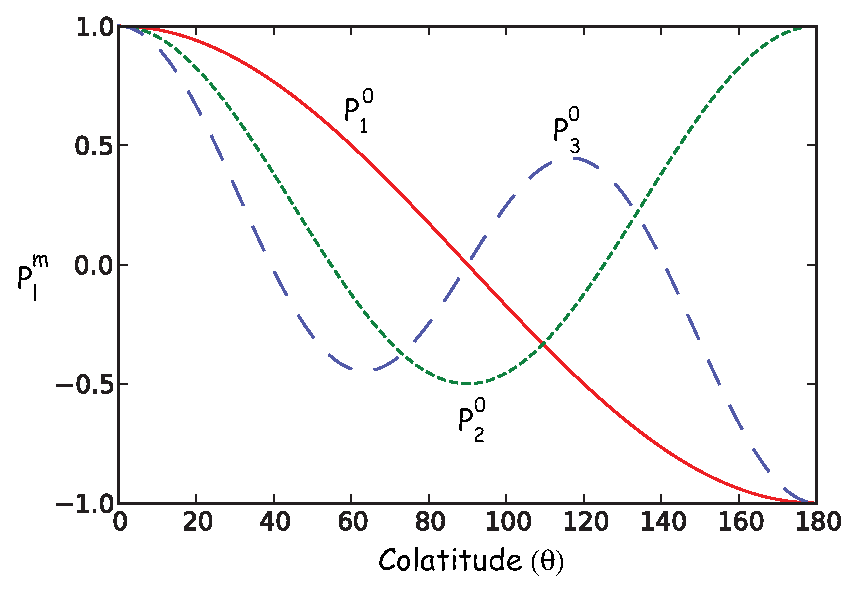
\includegraphics[width=11 cm]{EPSfiles/schmidt.eps}
\caption{Schmidt polynomials.}
\label{fig:schmidt}
\end{figure}


\index{spherical!harmonics}
To get an idea of how the  gauss coefficients in the potential relate to the associated magnetic fields, we show three examples 
 in  Figure~\ref{fig:harmonics}.  We plot the inclinations of the vector fields   that would be produced by the terms with $g_1^0, g_2^0$ and $g_3^0$ respectively.  
 \index{spherical!harmonics!dipole term}
 \index{spherical!harmonics!quadrupole term}
 \index{spherical!harmonics!octupole term}
 These are the axial ($m=0$)  dipole ($l=1$), quadrupole ($l=2$) and octupole ($l=3$) terms. 
The  associated potentials for each harmonic  are shown in the   insets.  
 
 \begin{figure}[htb]
%\epsfxsize 14.5cm
%\centering \epsffile{EPSfiles/harmonics.eps}
\centering  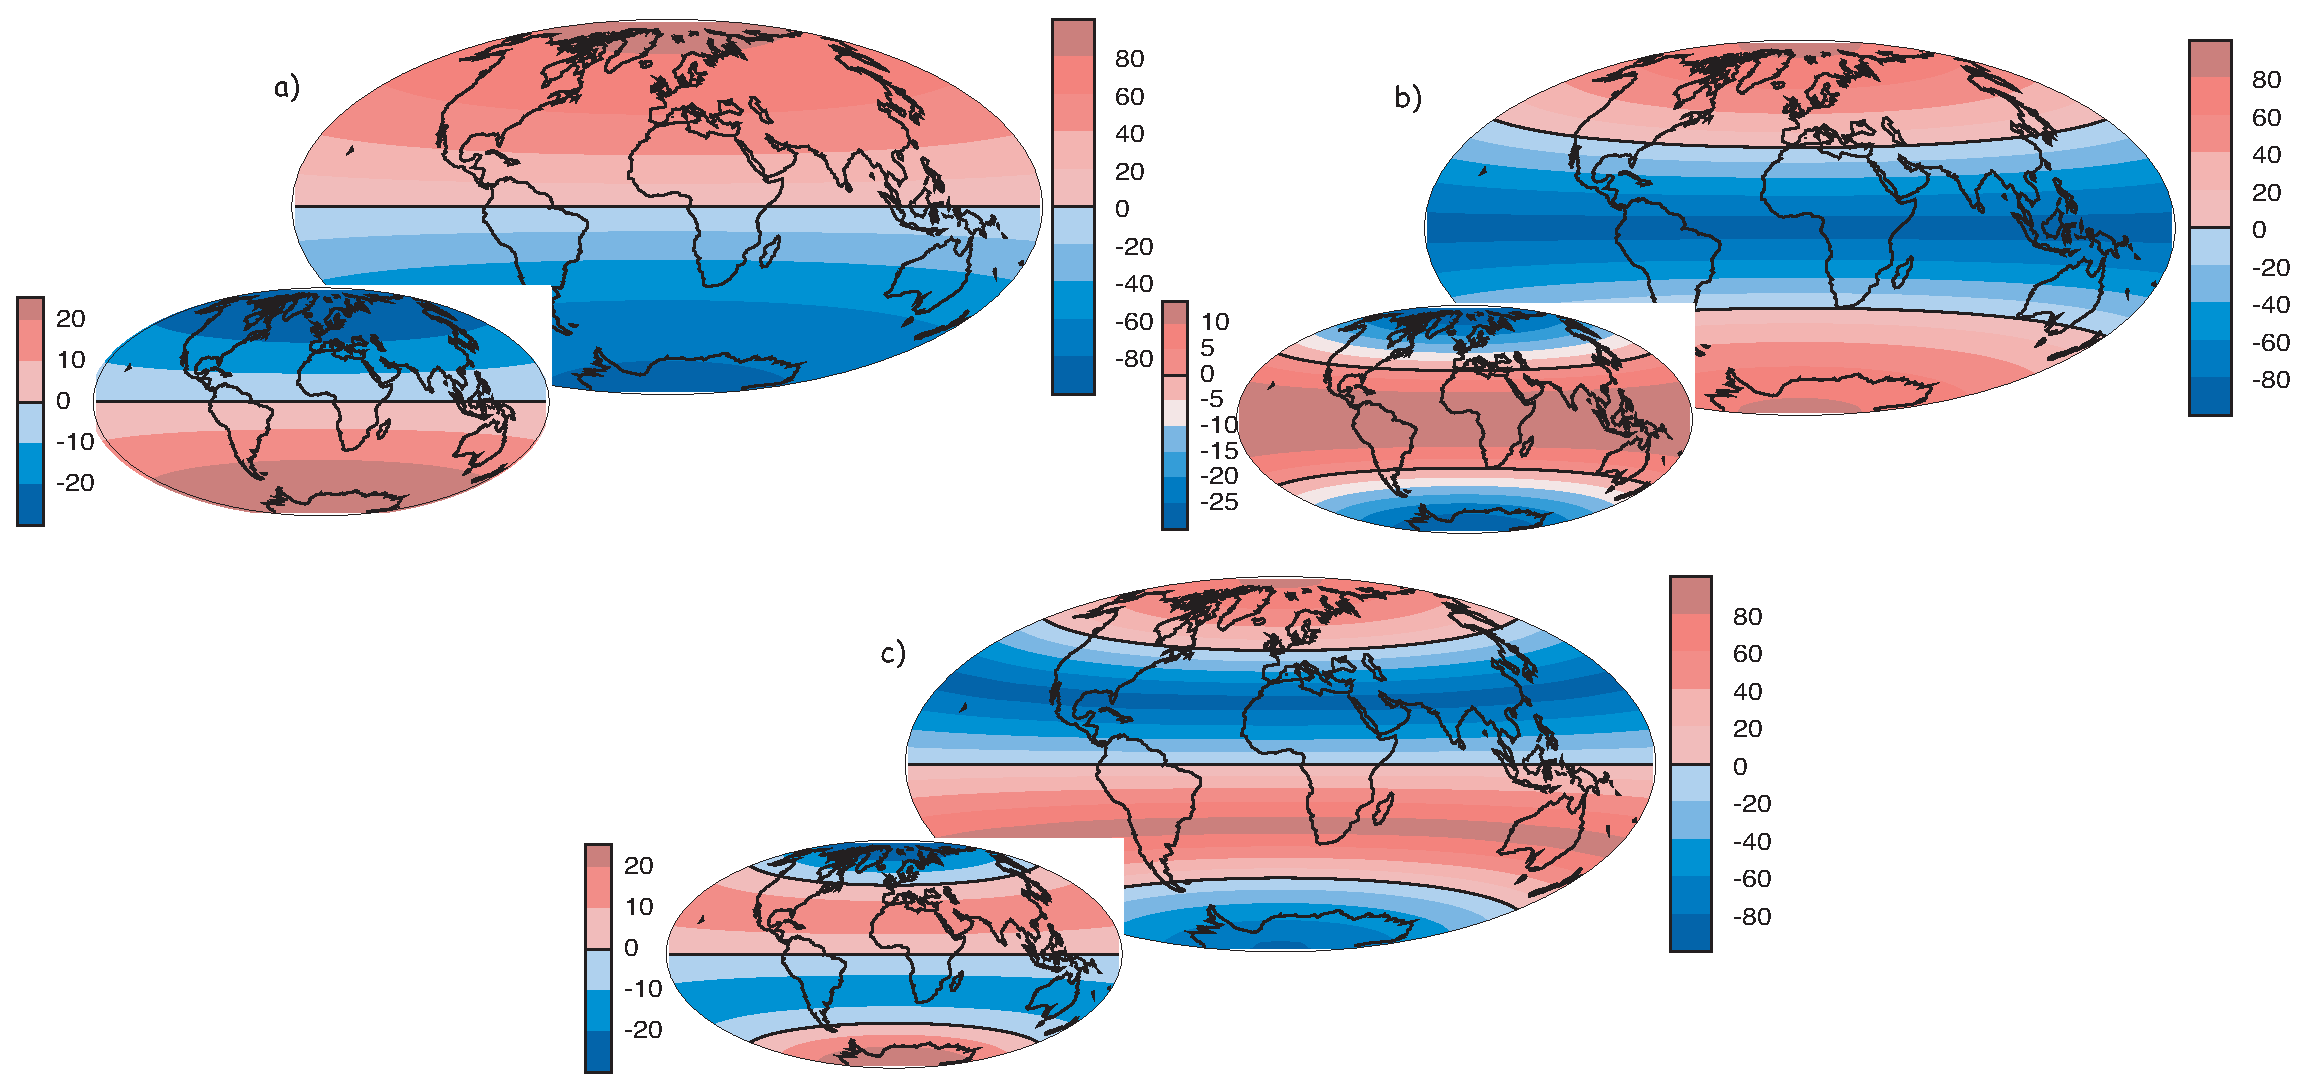
\includegraphics[width=14.5 cm]{EPSfiles/harmonics.eps}
\caption{Examples of potential fields (insets)  and maps of  the associated patterns for global inclinations.  Each coefficient is set to 30 $\mu$T.   a) Dipole ($g_1^0=30 \mu$T), b) Quadrupole ($g_2^0=30 \mu$T), c) Octupole ($g_3^0=30 \mu$T).    }
\label{fig:harmonics}
\end{figure}


  In general, terms for which the difference between the subscript ($l$) and the superscript ($m$) is odd (e.g., the axial dipole $g_1^0$ and octupole $g_3^0$)  produce magnetic fields that are antisymmetric about the equator, while those for which the difference is even (e.g., the axial quadrupole $g_2^0$) have symmetric fields.  In Figure~\ref{fig:harmonics}a we show the inclinations produced by a purely dipolar field of the same sign as the present day field.  The inclinations are all positive (down) in the northern hemisphere and negative (up) in the southern hemisphere.  In contrast, inclinations produced by a purely quadrupolar field (Figure~\ref{fig:harmonics}b) are down at the poles and up at the equator.    The map of inclinations produced by a purely axial octupolar field (Figure~\ref{fig:harmonics}c) are again asymmetric about the equator  with  vertical directions of opposite signs at the poles separated by bands with the opposite sign at mid-latitudes.    

As noted before, there is not one, but three dipole terms in Equation~\ref{eq:V},   the axial term ($g_1^0$) and two equatorial terms ($g_1^1$ and $h_1^1$).  
Therefore, the total dipole contribution is the vector sum of these three or $\sqrt{{g_1^0}^2+{g_1^1}^2+{h_1^1}^2}$.   The total quadrupole contribution ($l=2$) combines five coefficients and the total octupole ($l=3$)  contribution combines seven coefficients.  
 




So how do we get this marvelous list of gauss coefficients?  If you want to know the details, please refer Langel (1987). \nocite{langel87}  We will just give a brief introduction here.  
Recalling Chapter 1, once the scalar potential $\psi_m$ is known, 
the components of the magnetic field can
be calculated from it.  We solved this for the radial and tangential field components ($H_r$ and $H_{\theta}$)  in Chapter 1.   We will now change 
\index{coordinate systems}%
coordinate  and unit systems  and introduce a third dimension (because the field is not  perfectly dipolar).   The north, east, and vertically down components are related to the potential  $\psi_m$ by:

\begin{equation} 
B_N=-{\mu_o\over r}  {{\partial \psi_m} \over { \partial  \theta}},
 B_E=-{\mu_o\over {r \sin \theta }} {{\partial \psi_m} \over {\partial \phi}},
 B_V=-{\mu_o{\partial \psi_m} \over{ \partial r}}.
\label{eq:BnBeBv}
 \end{equation}


\noindent where $r$, $\theta$, $\phi$ are radius, co-latitude (degrees
away from the North pole) and longitude,
respectively. Here, $B_V$ is positive down, $B_E$ is positive east, and  $B_N$ is positive to the north, the opposite of
$H_r$ and $H_{\theta}$ as defined in Chapter 1. Note that
Equation~\ref{eq:BnBeBv} is in units of induction, not Am$^{-1}$ if the units for the gauss coefficients are in  nT, as is the current practice.     

Going backwards, 
the gauss coefficients  are determined by fitting 
Equations~\ref{eq:BnBeBv}
 and \ref{eq:V} to observations
of the magnetic field made by magnetic observatories or satellite for a particular time.
The {\it International (or Definitive) Geomagnetic Reference
Field}  or  I(D)GRF,  for a given time interval is an agreed upon set of values for a
number of gauss coefficients and their time derivatives.  
\index{Field models!IGRF}%
\index{Field models!IDGRF}%
IGRF (or DGRF) models and programs
for calculating various components of the magnetic field
are available on the internet from the 
National Geophysical Data Center; the address is \url{http://www.ngdc.noaa.gov}.  there is also a program {\bf igrf.py} included in the {\bf PmagPy} package (see \href{http://earthref.org/PmagPy/cookbook/#igrf.py}{igrf.py documentation}).   

In practice, the   gauss
coefficients for a particular reference field are estimated by least-squares fitting of  observations of the geomagnetic field.  You need a minimum of  48
observations to estimate the coefficients to $l=6$.  Nowadays, we have satellites which give us  thousands of measurements and the list of generation 10 of the IGRF for 2005 goes to $l=13$.  


\begin{table}[h!tb]
\begin{center}
\caption {IGRF,  12$^{th}$ generation (2015) to $l=6$. (Thebault et al., 2015)}
\label{tab:igrf15}
\begin{tabular}{r r r r|rrrr}
\hline
$l$&$m$&$g $( nT) &$h$ (nT) & $l$&$m$&$g $( nT) &$h$ (nT) \\
\hline
1 & 0 & -29442.0 & 0 & 5 & 0 & -232.6 & 0\\
1 & 1 & -1501.0 & 4797.1 & 5 & 1 & 360.1 & 47.3\\
2 & 0 & -2445.1 & 0 & 5 & 2 & 192.4 & 197.0\\
2 & 1 & 3012.9 & -2845.6 & 5 & 3 & -140.9 & -119.3\\
2 & 2 & 1676.7 & -641.9 & 5 & 4 & -157.5 & 16.0\\
3 & 0 & 1350.7 & 0 & 5 & 5 & 4.1 & 100.2\\
3 & 1 & -2352.3 & -115.3 & 6 & 0 & 70.0 & 0\\
3 & 2 & 1225.6 & 244.9 & 6 & 1 & 67.7 & -20.8\\
3 & 3 & 582.0 & -538.4 & 6 & 2 & 72.7 & 33.2\\ 
4 & 0 & 907.6 & 0 & 6 & 3 & -129.9 & 58.9\\
4 & 1 & 813.7 & 283.3 & 6 & 4 & -28.9 & -66.7\\
4 & 2 & 120.4 & -188.7 & 6 & 5 & 13.2 & 7.3\\
4 & 3 & -334.9 & 180.9 & 6 & 6 & -70.9 & 62.6\\ 
4 & 4 & 70.4 & -329.5 \\
 \hline
\end{tabular}
\end{center}
\end{table}
  \nocite{thebault15}


In order to get a feel for the importance of the various gauss coefficients, take a look at Table~\ref{tab:igrf15}, which has the Schmidt quasi-normalized gauss coefficients for the first six degrees from the IGRF for 2005.   
The power at each degree is the average squared field per spherical harmonic degree over the Earth's surface and is calculated by  $R_l=\sum_m (l+1)[(g_l^m)^2 + (h_l^m)^2]$
\index{Lowes, F.J.} \nocite{lowes74} 
(Lowes, 1974). 
The  so-called 
\index{Lowes spectrum}
{\it Lowes spectrum} is shown in 
Figure~\ref{fig:power}.  It is clear that the lowest order terms (degree one) totally
dominate,   constituting some 90\% of the field.    This is why the geomagnetic field is often assumed to be equivalent to a magnetic field created by a simple dipole at the center of the Earth.   



\begin{figure}[htb]
%\epsfxsize 11cm
%\centering \epsffile{EPSfiles/power.eps}
\centering  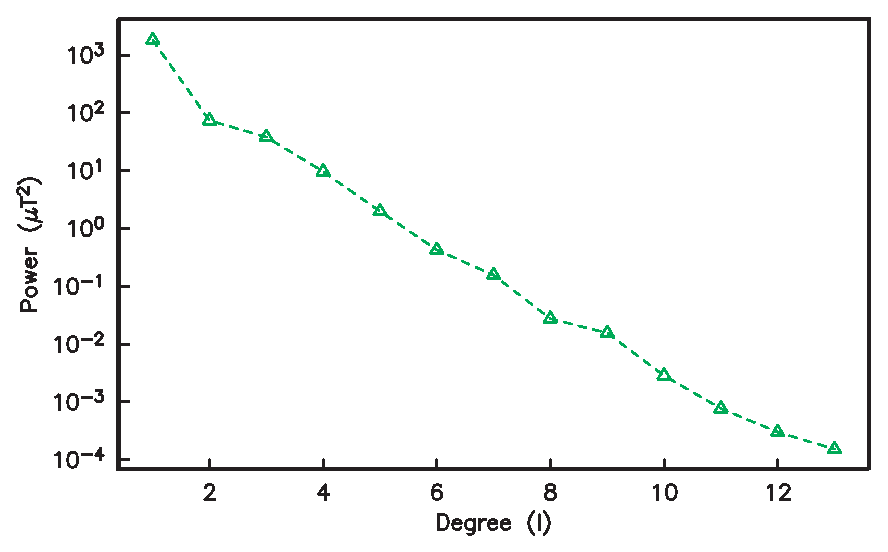
\includegraphics[width=11 cm]{EPSfiles/power.eps}
\caption{ Power at the Earth's surface of the geomagnetic field versus degree for the 2005 IGRF  (Table 2.1). }
\label{fig:power}
\end{figure}



\begin{figure}[htb]
 %\epsfxsize  14cm
%\centering \epsffile {EPSfiles/B.eps}
\centering  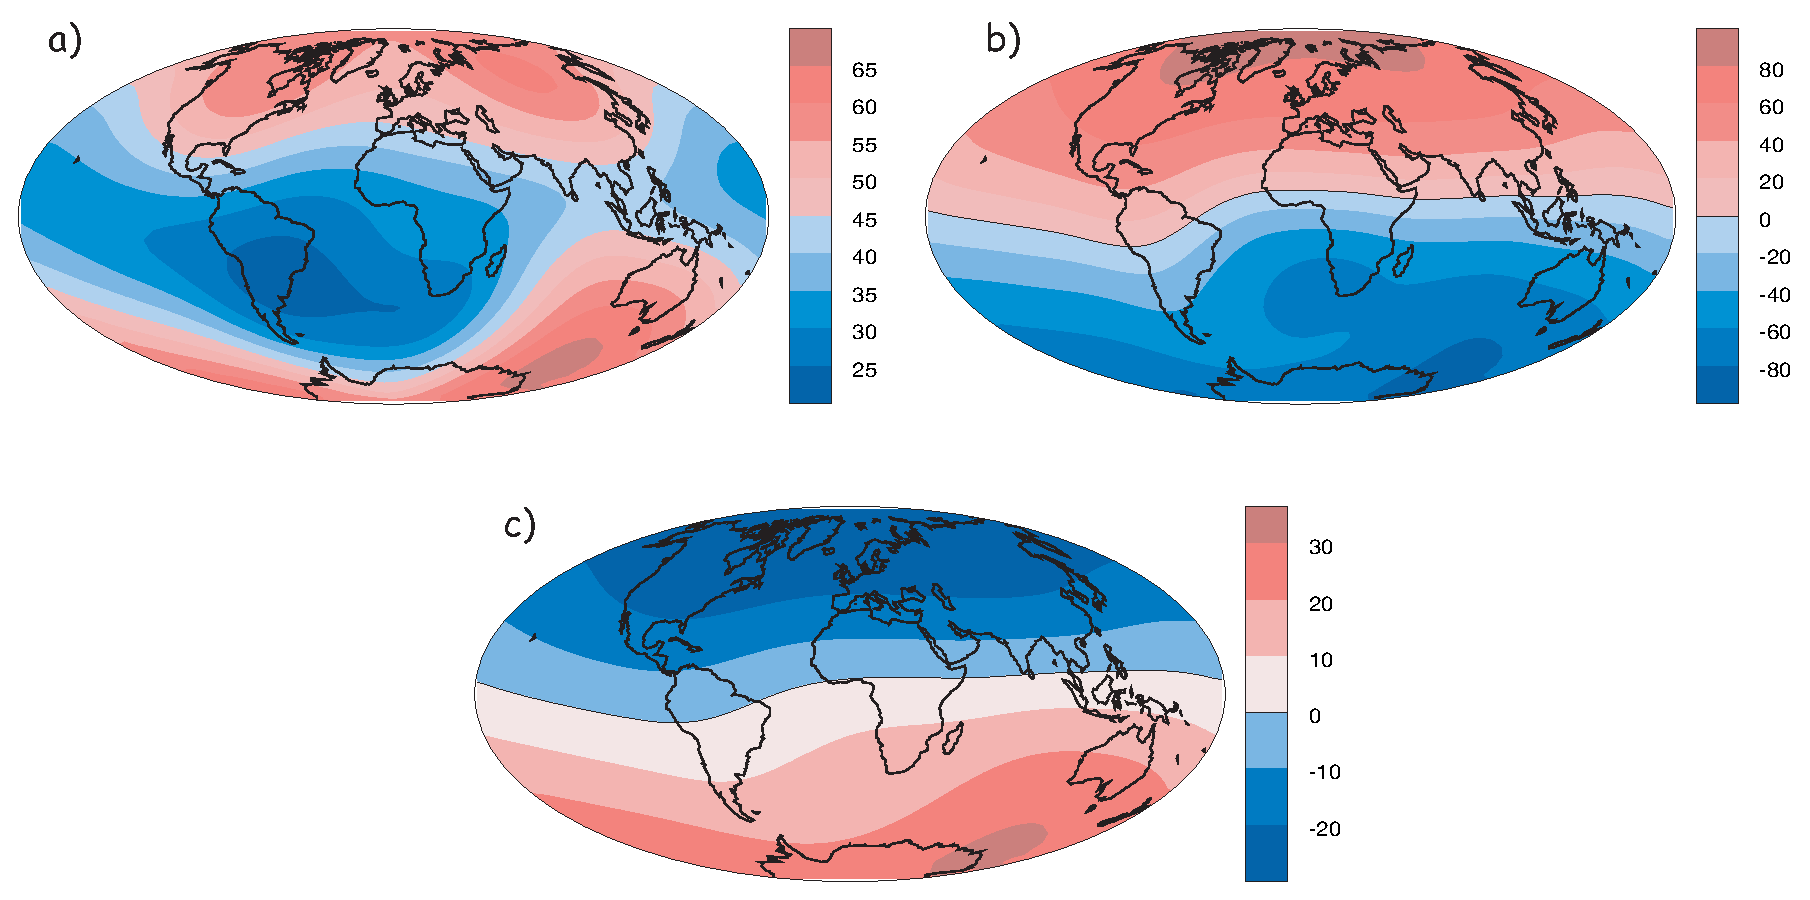
\includegraphics[width=14 cm]{EPSfiles/B.eps}
\caption {Maps of geomagnetic field of the IGRF for 2005.
a) Intensity (units of $\mu$T), b) inclination, c) potential (units of nT).}
\label{fig:B}
\end{figure}



\section{Geocentric axial dipole (GAD) and other poles}
\label{sect:gad}

The beauty of using the geomagnetic potential field is that the vector field can be evaluated anywhere outside the source region.      Using the 
values for a given reference field in   
  Equations~\ref{eq:V} and \ref{eq:BnBeBv}, we can   calculate
 values of $B, D$ and $I$ at any location on Earth.    Figure~\ref{fig:coord}b shows the lines of flux predicted from the 2005 IGRF from  the core-mantle boundary up.   We can see that the field becomes simpler and more dipolar as we move from the core mantle boundary to the surface.  Yet, there is still significant non-dipolar structure in the geomagnetic field even at the Earth's surface.  
 
   We can recast the vectors at the surface of the Earth into  maps of components as  shown in 
Figure~\ref{fig:B}a,b.   
We show the potential in Figure~\ref{fig:B}c for comparison with that of  a pure dipole (inset to Figure~\ref{fig:harmonics}a).      These maps illustrate the fact that
the field is a complicated function of position on the surface of the Earth.  
The intensity values in Figure~\ref{fig:B}a are, in
general,  highest near the poles ($\sim$ 60 $\mu$T) and lowest near the equator
($\sim$ 30 $\mu$T), but the contours are not straight lines parallel to latitude
as they would be for a field generated strictly by a 
\index{Field models!geocentric axial dipole}
geocentric axial dipole (GAD) (e.g, Figure~\ref{fig:coord}a).  
 Similarly, a GAD would produce lines of 
inclination that vary in a regular way from -90$^{\circ}$ to +90$^{\circ}$
at the poles, with 0$^{\circ}$ at the equator;  the contours
would parallel the lines of latitude.  Although the general trend in inclination
shown in Figure~\ref{fig:B}b is similar to the GAD model, the field lines are more complicated, which again suggests that the field is not perfectly
described by a geocentric bar magnet. 





\begin{figure}[htb]
%\epsfxsize 9cm
%\centering \epsffile{EPSfiles/poles.eps}
\centering  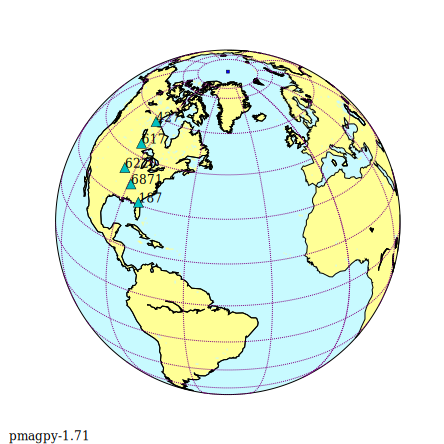
\includegraphics[width=9 cm]{EPSfiles/poles.eps}
\caption{Different poles.  
The square is the magnetic North Pole, where the magnetic field is straight
down $(I = +90^{\circ})$ (82.7$^{\circ}$N, 114.4$^{\circ}$W for  the IGRF 2005); the circle is the geomagnetic North Pole, where the axis of the
best fitting dipole pierces the surface (9.7$^{\circ}$N, 71.8$^{\circ}$W for the  IGRF 2005). 
 The star is the geographic North Pole.  [Figure made using Google Earth with seafloor topography of  D. Sandwell supplied to Google Earth by  D. Staudigel.]}
\label{fig:poles}
\end{figure}




Perhaps the most important result of
\index{spherical!harmonics}%
spherical harmonic analysis for our purposes is that the field at the Earth's surface is dominated
by the degree one terms ($l=1$) and the external contributions are very
small.
  The first order terms can be thought of as geocentric dipoles that are aligned
with three different axes: the spin axis ($g_1^0$) and two equatorial axes 
that intersect the equator at the Greenwich meridian 
($h_1^0$) and at 90$^{\circ}$ East ($h_1^1$).               
\index{pole!geomagnetic}%
\index{geomagnetic!pole}%
The vector sum of these geocentric dipoles  is a dipole that is currently
 inclined by about 10$^{\circ}$ to the spin axis.  The
axis of this {\it best-fitting dipole} pierces the surface of the Earth at the circle in
Figure~\ref{fig:poles}.  This point and its antipode are called
 {\it geomagnetic poles}.  Points at which the field
is vertical ($I = \pm 90^{\circ}$ shown by a square in Figure~\ref{fig:poles}) are called  
{\it magnetic poles}, or sometimes 
\index{pole!magnetic}%
\index{magnetic!pole}%
\index{pole!dip}%
\index{dip pole}%
{\it dip poles}.  These poles are distinguishable from the {\it geographic poles},
  where the spin axis of the Earth intersects its surface.
The northern geographic pole is shown by a star in Figure~\ref{fig:poles}.

\index{pole!geographic}%
\index{geographic pole}%
It turns out that when averaged over sufficient time, the geomagnetic field  actually does seem  to be  approximately  a GAD field, perhaps with a pinch of $g_2^0$ thrown in
\index{Merrill, R.T.} \nocite{merrill96}
 (see e.g., Merrill et al., 1996). 
The GAD model of the field will serve as a useful crutch 
throughout our discussions of
paleomagnetic data and applications. 
Averaging ancient magnetic poles over enough time to average out secular variation (thought to be  10$^4$ or 10$^5$ years)  gives what is known
as a 
\index{pole!paleomagnetic}%
{\it paleomagnetic pole}; this  is usually assumed to be co-axial with the Earth's geographic pole (the spin axis).  


Because the geomagnetic field is axially dipolar 
to a  first approximation, we can write:

\beq \psi_m= {a\over{\mu_o} }g_1^0 \left({a \over r} \right)^2 P_1^0 ( \cos \theta ) = {a\over{\mu_o} } g_1^0
\left( {a \over r} \right)^2 \cos \theta.
\label{eq:Vmdip}
\eeq

 Note that $g_1^0$ is given in nT in Table~\ref{tab:igrf15}.    Thus, from Equation~\ref{eq:Vmdip}, 

\begin{equation} 
{B_N}=\mu_o H_N= {g_1^0 a^3 \sin \theta \over r^3}, \hskip 1em B_E=0, \hskip 1em \hbox{and} \hskip 1em
 B_V=\mu_o H_V=  {2 g_1^0 a^3 \cos \theta
\over r^3}.
\label{eq:Bnevdip}
 \end{equation}

\noindent Given some latitude $\lambda$
 on the surface of the Earth 
 in  Figure~\ref{fig:coord}a
and using the equations for $B_V$ and $B_N$, we find that:

\begin{equation} \tan  I = {B_V \over B_N} = 2 \cot  
\theta = 2 \tan \lambda.
\label{eq:dipform}
 \end{equation} 

\index{dipole!formula}%
\index{dipole!equation}%
\noindent This equation is sometimes called the {\it dipole formula}  and
shows that the inclination of the magnetic field
 is directly related to the co-latitude  ($\theta$) for a
 field produced by a geocentric axial dipole (or $g_1^0$). The dipole formula allows us to
calculate the latitude of the measuring position from the inclination of the
(GAD) magnetic field, a result that is fundamental in plate tectonic reconstructions. 
The intensity of a dipolar magnetic 
field is also related to (co)latitude because:

\beq 
 B = (B_V^2 + B_N^2 )^\half
= {g_1^0 a^3 \over r^3} ( \sin^2 \theta + 4 \cos^2 \theta)^{1\over 2}
 = {g_1^0 a^3 \over r^3} ( 1 + 3 \cos^2 \theta)^\half.
\label{eq:Bvdip}
\eeq

\noindent The dipole field intensity has changed by more than an order of magnitude 
in the past and the dipole relationship of intensity to latitude
 turns out to be not useful for tectonic reconstructions.  

 

\section{Plotting magnetic directional data}
\label{sect:eqarea}


Magnetic field and magnetization directions 
can be visualized as unit vectors anchored at the center of
a unit sphere. Such a unit sphere is difficult to represent on a 2-D page.
There are several popular projections, including the
Lambert equal area projection which we will be making extensive use
of  in later chapters.  The principles of
construction of the equal area projection 
are covered in the Appendix~\ref{app:eqarea}.

In general, regions of equal area on the sphere project as equal
area regions on this projection, as the name implies.  
Plotting directional data in this way  enables rapid
assessment of data scatter.  A drawback
of this projection is that circles 
on the surface of a sphere project as ellipses.  Also, because we have
projected a vector onto a unit sphere, we have lost
information concerning the magnitude of the vector.
Finally, lower and upper hemisphere projections must be distinguished
with different symbols.  The paleomagnetic  convention is:
lower hemisphere projections (downward directions)  use solid
symbols, while upper hemisphere projections
are open. 

\begin{figure}[htb]
%\epsfxsize 11cm
%\centering \epsffile{EPSfiles/igrf.eps}
\centering  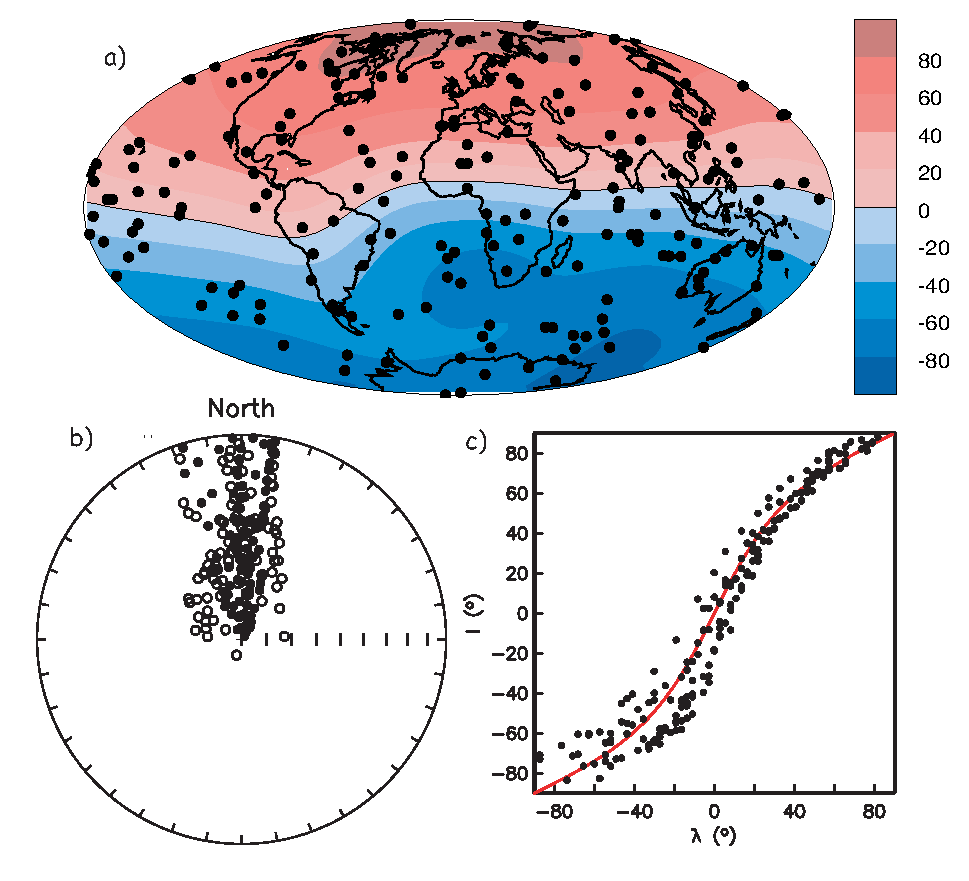
\includegraphics[width=11 cm]{EPSfiles/igrf.eps}
\caption{
a) Hammer projection of 200 randomly selected locations around the globe.
b) Equal area projection of directions of Earth's magnetic field as given 
by the
IGRF evaluated for the year 2005 at locations shown in a). Open (closed)
symbols indicate upper (lower) hemisphere. c) Inclinations
(I) plotted as a function of site latitude ($\lambda$). 
The solid line is the inclination
expected from the dipole formula (see text). Negative latitudes are
south and negative inclinations are up. [Figure redrawn from Tauxe, 1998.]}
\label{fig:igrf}
\end{figure}
\nocite{tauxe98}


The dipole formula allows us to convert a given measurement of $I$ to an equivalent
\index{magnetic!colatitude}
 {\it magnetic
co-latitude} $\theta_m$:

\beq
\cot \theta_m = \half \tan I.
\label{eq:mcolat}
\eeq

If the field were a simple GAD field,  $\theta_m$ would be a reasonable estimate of
$\theta$, but non-GAD terms can invalidate this assumption.   To get a feel for the effect of these non-GAD terms, we
consider first what would happen if we took random measurements of the
Earth's present field (see Figure \ref{fig:igrf}).  We evaluated the 
directions of the magnetic field  using the IGRF for 
2005 at   200 positions on the globe (shown in 
Figure~\ref{fig:igrf}a).  These directions are plotted in
Figure~\ref{fig:igrf}b using the paleomagnetic convention 
of open symbols pointing up and closed symbols pointing down.  
In
Figure~\ref{fig:igrf}c, we plot the inclinations as a function of latitude.
As expected from a predominantly dipolar field, 
inclinations cluster around the values for a geocentric axial
dipolar field but there is considerable scatter and interestingly the scatter is larger in the southern hemisphere than in the northern one.   This is related to the low intensities beneath South America and the Atlantic region seen in Figure~\ref{fig:B}a. 

\subsection{$D', I' $ transformation}  

Often we wish to compare directions from distant parts of the globe.  There is an inherent difficulty in doing so because of the large variability in inclination with latitude.  
In such cases it is appropriate to  consider the data relative to the expected direction (from GAD) at each sampling 
site.  For this purpose, it is useful to use a transformation   
whereby each direction is rotated such that the  direction expected from a
geocentric axial dipole field (GAD) at the sampling site is the center of the equal 
area projection.  This is accomplished as follows:

Each direction is converted to Cartesian coordinates ($x_{i}$) by:

\begin{equation}
x_{1}= \cos D \cos I; \hskip 1em
x_{2}= \sin D \cos I; \hskip 1em x_{3}= \sin I.
\label{eq:dir2cart}
\end{equation}

\noindent
These are rotated to the new coordinate system ($x'_{i}$, see Appendix~\ref{app:tensors}) by:
$$
x'_{1}= (x_{1}^{2}+x_{3}^{2})^{1/2} \sin (I_{d} - \alpha); \hskip 1em
x'_{2}=x_{2}; \hskip 1em
x'_{3}=(x_{1}^{2}+x_{3}^{2})^{1/2} \cos (I_{d} - \alpha),
$$

\noindent
where $I_{d}$ = the inclination expected from a GAD field ($\tan 
I_{d}=2\tan \lambda$),  $\lambda$ is the site latitude, and $\alpha $ 
is the inclination of the paleofield vector projected onto the N-S 
plane ($\alpha = \tan^{-1} (x_{3}/x_{1})$).   The $x'_{i}$ are then 
converted to $D',I'$ by Equation~\ref{eq:DI}. 

In Figure~\ref{fig:didip}a we show the geomagnetic field vectors evaluated at random longitudes along a latitude band of 45$^{\circ}$N.  The vectors are shown in their Cartesian coordinates of North, East and Down.  In Figure~\ref{fig:didip}b we show what happens when we rotate the coordinate system to peer down the direction expected from an axial dipolar field at 45$^{\circ}$N (which has an inclination of 63$^{\circ}$).    The vectors circle about the expected direction.    Finally,   
we see what happens to the directions shown in 
Figure~\ref{fig:igrf}b after the $D',I'$ transformation in Figure~\ref{fig:didip}.   These are unit vectors projected along the expected direction for each observation  in Figure~\ref{fig:igrf}a.   Comparing the equal area projection of the directions themselves (Figure~\ref{fig:igrf}b) to the transformed directions (Figure~\ref{fig:didip}c), we see that the latitudal dependence of the inclinations has been removed. 

\begin{figure}[htb]
%\epsfxsize 14cm
%\centering \epsffile{EPSfiles/igrf.dip.eps}
\centering  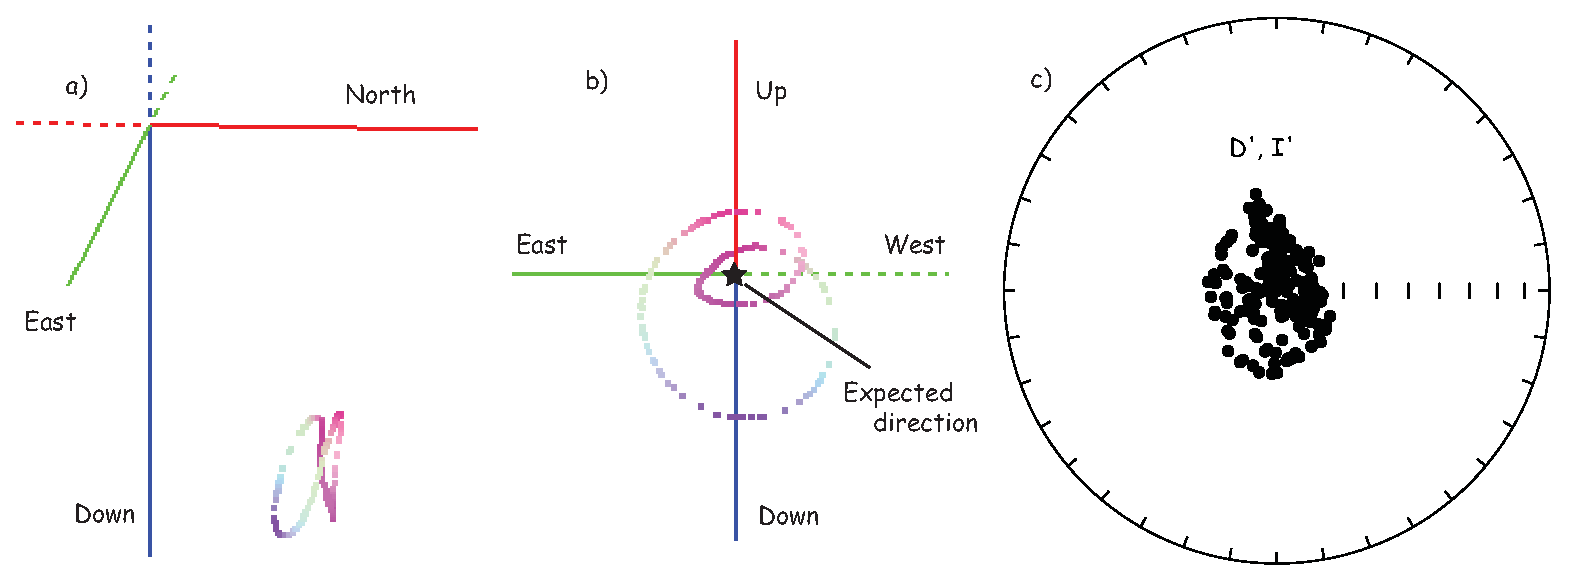
\includegraphics[width=14 cm]{EPSfiles/igrf_dip.eps}
\caption{a) Vectors evaluated around the globe at 45$^{\circ}$N.  Red/green/blue colors reflect the North, East and Down components respectively.  b) The unit vectors  (assuming unit length) from a).  c) Directions from Figure 2.7b transformed using the $D', I'$ transformation.}
\label{fig:didip}
\end{figure}


\begin{figure}[!htb]
%\epsfxsize 13cm
%\centering \epsffile{EPSfiles/mkvgp.eps }
\centering  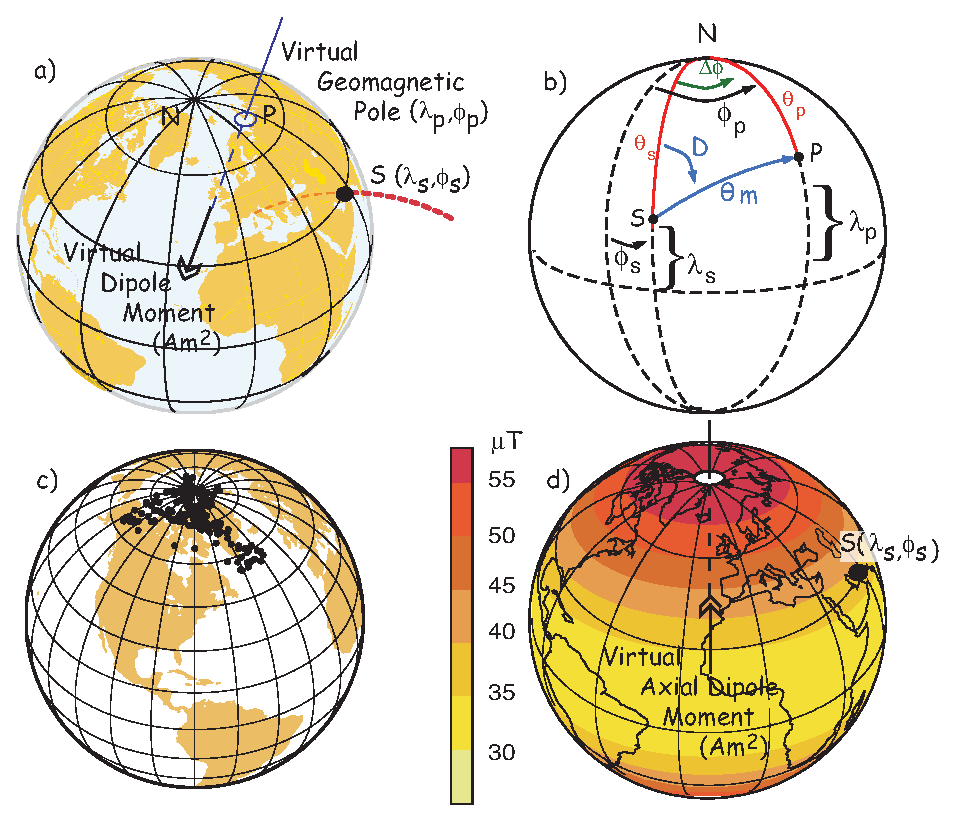
\includegraphics[width=13 cm]{EPSfiles/mkvgp.eps}
\caption {Transformation of a vector measured at S into a virtual
geomagnetic pole position (VGP) and virtual dipole moment (VDM),
using principles of spherical trigonometry and the dipole formula.  a) Red dashed line is the magnetic field line  observed at S (latitude of $\lambda_s$, longitude of $\phi_s$).  This field line is the  same as one produced by the VDM at the center of the Earth.  The point where the axis of the  VDM pierces the Earth's surface is the VGP.    b)  Observed declination (D) and inclination (converted to $\theta_m$ using the dipole formula (see text) defines angles $D$ and $\theta_m$.  $\theta_s$ is the colatitude of the observation site. N is the geographic North Pole (the spin axis of
the Earth). The position of the pole at P ($\theta_p,\phi_p$)  can be calculated with spherical trigonometry (see text).    c) VGP positions converted from directions shown in Figure 2.7b. d) The virtual axial dipole moment giving rise to the observed intensity at S.}
\label{fig:mkvgp}
\end{figure}

\customlink{Virtual_geomagnetic_poles}
\subsection{Virtual geomagnetic poles}
\label{sect:vgp}

 We are often interested in
whether the geomagnetic pole has changed, or whether a particular piece of crust
has rotated with respect to the geomagnetic pole.  Yet, what we
observe at a particular location is the local direction of the field
vector.  Thus, we need a way to transform an observed direction into the
equivalent geomagnetic pole. 

In order to remove the dependence of direction merely on position 
on the globe,  we imagine a geocentric dipole which would
give rise to the observed magnetic field direction
 at a given latitude ($\lambda$) and
longitude ($\phi$).  
\index{pole!virtual geomagnetic}%
\index{virtual!geomagnetic pole}%
The {\it virtual geomagnetic pole} (VGP) is the point
on the globe that corresponds to the geomagnetic pole of this imaginary dipole 
(Figure~\ref{fig:mkvgp}a).

Paleomagnetists use the following conventions:   $\phi$  is measured
positive eastward from the Greenwich meridian and
ranges from $0 \rightarrow 360^\circ$;  $\theta $  is measured  from
the North pole and goes from $0 \rightarrow 180^\circ$. Of course
$\theta $ relates
to latitude, $\lambda $ by $\theta = 90 - \lambda $.  $\theta_m$ is the
magnetic co-latitude and is given by Equation~\ref{eq:mcolat}. 
Be sure not to confuse latitudes and co-latitudes.
Also, be careful with 
\index{magnetic!declination}%
declination.  Declinations between 180$^\circ$
and 360$^{\circ}$ are equivalent to $D$ - 360 $^\circ$ which are
counter-clockwise with respect to North.  

The first step in the problem  of calculating a VGP is to determine the
\index{magnetic!colatitude}%
 magnetic co-latitude $\theta_m$ by Equation~\ref{eq:mcolat} which is defined in the dipole formula (Equation~\ref{eq:mcolat}).
The declination $D$ is the angle from the geographic
North Pole to the
great circle joining the observation site $S$ and the pole $P$, and $\Delta \phi$ is the difference
in longitudes between P and S, 
$\phi_p-\phi_s$.  Now we use some tricks from 
\index{spherical!trigonometry}%
spherical trigonometry as reviewed in Appendix~\ref{app:strig}.

 
We can  locate VGPs using the law of sines and the law of cosines. 
The 
\index{magnetic!declination}
declination $D$ is the angle from the geographic North Pole
to the
great circle joining $S$ and $P$ (see Figure~\ref{fig:mkvgp}) so:
 
\def\pih{{\pi \over 2}}
\beq \cos \theta_p = \cos \theta_s  \cos
\theta_m + \sin \theta_s \sin \theta_m \cos D, 
\label{eq:vgplat}
\eeq
 
\noindent which allows us to calculate the VGP co-latitude $\theta_p$. The
VGP latitude is given by:

$$
\lambda_p = 90 - \theta_p,
$$
\noindent so $90>\lambda_p>0$ in the northern hemisphere and
$0<\lambda_p<90$ in the southern hemisphere.
 
To determine $\phi_p$, we first calculate the angular difference between
the pole and site
longitude $\Delta \phi$.  
 
\beq {{\sin \Delta \phi}=  \sin \theta_m} \cdot { \sin D \over
\sin \theta_p } .
\label{eq:vgplong}
\eeq
 
\noindent  If $\cos \theta_m
\geq \cos \theta_s \cos \theta_p$, then $\phi_p = \phi_s+\Delta \phi$.
However, if $\cos \theta_m <
\cos \theta_s \cos \theta_p$ then
$\phi_p=\phi_s + 180 -\Delta \phi$.


Now we can convert the directions in
Figure~\ref{fig:igrf}b to 
\index{virtual!geomagnetic pole}%
VGPs (see Figure~\ref{fig:mkvgp}c).  The grouping 
of points is much tighter in Figure~\ref{fig:mkvgp}c than in the
equal area projection because the effect
of latitude variations in dipole fields has been removed.    
If a number of VGPs are averaged together, the average pole position is called a ``paleomagnetic pole''.  How to average poles and directions is the subject of Chapters 11 and 12.

The procedure for calculating a direction from a VGP is a similar procedure to that for calculating the VGP from the direction.    
\index{magnetic!colatitude}
Magnetic colatitude $\theta_m$ is calculated in exactly the same way as before and yields inclination from the dipole formula.   The declination can be calculated  by solving for $D$ in Equation~\ref{eq:vgplat} as:

$$
\cos D = { { \cos \theta_p - \cos \theta_s \cos \theta_m} \over { \sin \theta_s \sin \theta_m} }.
$$

\noindent
This equation works most of the time, but breaks down under some circumstances, for example, when the pole latitude is further to the south than the site latitude.   The following algorithm works in the more general case:



$$
D= - \tan^{-1} (  { { \cos D}\over { \sqrt{ C}  } }) + 90,
$$
\noindent where $C = |1- (\cos D)^2|$.     Also, if  $-90 < \Delta \phi <0$ or if $ \Delta \phi > 180$, then $D = 360 - D$.       
 
\index{virtual!dipole moment}%
\customlink{Virtual_dipole_moment}
\subsection {Virtual dipole moment}
\label{sect:vdm}

As pointed out earlier,  magnetic
intensity varies
 over the globe in a similar manner to inclination.   It is 
 often convenient to express
paleointensity values in terms of the equivalent geocentric dipole
moment
that would have produced the observed intensity at a specific  (paleo)latitude.
Such an equivalent  moment is called the {\it virtual dipole moment} (VDM) by
analogy to the VGP (see Figure~\ref{fig:mkvgp}a).  First, the magnetic
(paleo)co-latitude $\theta_m $ is calculated as before from the observed
inclination
and the dipole formula of Equation~\ref{eq:dipform}. Then, following the
derivation of Equation~\ref{eq:Bvdip}, we have

\beq \hbox {VDM} = {{4\pi r^3\over \mu_o} {{B}_{ancient}}
{{(1 + 3\cos^2 \theta_m)^{-{1\over 2}}}}}. 
\label{eq:vdm}
\eeq

\noindent Sometimes the site co-latitude as opposed to magnetic co-latitude
 is used in the above equation, giving a 
 \index{virtual!axial dipole moment}%
{\it virtual axial dipole moment} (VADM; see Figure~\ref{fig:mkvgp}d).

\vskip .5 in\noindent{SUPPLEMENTAL READINGS:} Merrill et al. (1996), Chapters 1 \& 2

\vskip 24pt
{\parindent 0pt \parskip 12pt 
\section{Problems}
 
For this and future problem sets, you will need the {\bf PmagPy}  package (see section in the Preface at the beginning of the book).  After you have installed this and properly set your path, you can import the functions from {\bf PmagPy} using these commands: 

\begin{verbatim}
import pmagpy.pmag as pmag
import pmagpy.ipmag as ipmag
import pmagpy.pmagplotlib as pmagplotlib
\end{verbatim}

Please consult the Jupyter notebook {\it PmagPy.ipynb} for more help  on using PmagPy functions within a notebook.  


{\bf Problem 1}


a) Write a python script in an Jupyter notebook
that converts
declination, inclination and intensity to North, East, and Down.   Read in the data in the file {\it Chapter\_2/ps2\_prob1\_data.txt}.  For this the {\bf loadtxt} function in the Numpy module will come in handy.   


b) Choose 10 random spots on the surface of the earth.  You can use the {\bf pmag.get\_unf} to generate a list for you.  Then 
use the {\bf ipmag.igrf} function   to  evaluate  the declination, inclination and intensity at each of these locations in January 2006.  As with all {\bf PmagPy} programs, and functions, you can find out what they do by printing out the doc string:
 you can find out what they do by getting the help message:

\begin{verbatim}
help(ipmag.igrf)
\end{verbatim}

\noindent  Calls like these generates  help messages which will help you to call the function properly.  



c) Take the vectors from the output of  Problem 1b and convert them to cartesian coordinates, using the  script you wrote in Problem 1a.  


{\bf Problem 2}

a) Plot the IGRF directions from Problem 1b  on an equal area projection by hand.    Use the equal area net provided in the Appendix.   Remember that the outer rim is  horizontal and the center of the diagram is vertical.  Azimuth goes around the rim with clockwise being positive.    Put a  thumbtack through the equal area (Schmidt) net and place a piece of tracing paper on the thumbtack. Mark the top of the stereonet with a tick mark on the tracing paper. 

To plot a direction,   rotate the tick mark of the tracing paper around  counter clockwise until the top of the paper is rotated by the declination of the direction. Then count tick marks toward the center from the outer rim (the horizontal) to the inclination angle, plot the point, and rotate back so that the tick is North again. Put all your points on the diagram.


b) Now use the {\bf ipmag} functions {\bf plot\_net } and {\bf plot\_di}.
 or write your own!  Both plots should look the same....


{\bf Problem 3}

You went to Wyoming (112$^{\circ}$ W and 36$^{\circ}$ N) to sample some Cretaceous rocks.  You measured a direction with a declination of 345$^{\circ}$ and an inclination of 47$^{\circ}$.  

a) What direction would you expect  from the present (GAD) field? 

b)  What is the virtual geomagnetic pole position corresponding to the direction you actually measured?  [Hint: Use the function {\bf pmag.dia\_vgp} in the {\bf PmagPy} module or for a challenge, write your own! ]



 


%
